%%%%%%%%%%%%%%%%%%%%%%%%%%%%%%%%%%%%%%%%%
% Class Notes Template
% LaTeX Template
% By: Ryan Grove
%%%%%%%%%%%%%%%%%%%%%%%%%%%%%%%%%%%%%%%%%

%----------------------------------------------------------------------------------------
%	PACKAGES AND OTHER DOCUMENT CONFIGURATIONS
%----------------------------------------------------------------------------------------

\documentclass[paper=a4, fontsize=11pt]{scrartcl} % A4 paper and 11pt font size

\usepackage[T1]{fontenc} % Use 8-bit encoding that has 256 glyphs
\usepackage{fourier} % Use the Adobe Utopia font for the document - comment this line to return to the LaTeX default
\usepackage[english]{babel} % English language/hyphenation
\usepackage{amsmath,amsfonts,amsthm} % Math packages

\usepackage{lipsum} % Used for inserting dummy 'Lorem ipsum' text into the template

\usepackage{sectsty} % Allows customizing section commands
\allsectionsfont{\centering \normalfont\scshape} % Make all sections centered, the default font and small caps

\usepackage{fancyhdr} % Custom headers and footers
\pagestyle{fancyplain} % Makes all pages in the document conform to the custom headers and footers
\fancyhead{} % No page header - if you want one, create it in the same way as the footers below
\fancyfoot[L]{} % Empty left footer
\fancyfoot[C]{} % Empty center footer
%\fancyfoot[R]{\thepage} % Page numbering for right footer
\renewcommand{\headrulewidth}{0pt} % Remove header underlines
\renewcommand{\footrulewidth}{0pt} % Remove footer underlines
\setlength{\headheight}{13.6pt} % Customize the height of the header

\numberwithin{equation}{section} % Number equations within sections (i.e. 1.1, 1.2, 2.1, 2.2 instead of 1, 2, 3, 4)
\numberwithin{figure}{section} % Number figures within sections (i.e. 1.1, 1.2, 2.1, 2.2 instead of 1, 2, 3, 4)
\numberwithin{table}{section} % Number tables within sections (i.e. 1.1, 1.2, 2.1, 2.2 instead of 1, 2, 3, 4)

\setlength\parindent{0pt} % Removes all indentation from paragraphs - comment this line for an assignment with lots of text

\usepackage{lastpage}
\usepackage{fancyhdr}
\cfoot{\thepage\ of \pageref{LastPage}}

\def\v{\hbox{$\mathbf v$}}
\def\w{\hbox{$\mathbf w$}}
\def\u{\hbox{$\mathbf u$}}
\def\x{\hbox{$\textbf{x}$}}
\def\z{\hbox{$\mathbf z$}}
\def\a{\hbox{$\mathbf a$}}
\def\b{\hbox{$\mathbf b$}}
\def\L{\hbox{$\mathcal L$}}
\def\C{\hbox{$\mathbb C$}}
\def\B{\hbox{$\mathcal B$}}
\def\R{\hbox{$\mathbb R$}}
\def\X{\hbox{$\underline X$}}
\def\Q{\hbox{$\mathbb Q$}}
\def\R{\hbox{$\mathbb R$}}
\def\N{\hbox{$\mathbb N$}}
\def\C{\hbox{$\mathbb C$}}
\def\0{\hbox{$\mathbf 0$}}
\def\Y{\hbox{$\underline Y$}}
\def\a{\hbox{$\mathbf a$}}
\def\u{\hbox{$\mathbf u$}}
\def\w{\hbox{$\mathbf w$}}
\def\y{\hbox{$\mathbf y$}}
\def\X{\hbox{$\underline X$}}
\def\dd{\hbox{$\partial $}}
\def\B{\hbox{$\mathcal B$}}
\def\F{\hbox{$\mathcal F$}}
\def\L{\hbox{$\mathcal L$}}
\def\M{\hbox{$\mathcal M$}}
\def\D{\hbox{$\mathscr {D}$}}
\def\RR{\hbox{$\mathscr{R}$}}
\def\I{\hbox{$\mathcal I$}}

\usepackage{amssymb}
%\theoremstyle{plain}
\usepackage[margin = .75in]{geometry}
\newtheorem{claim}{Claim}
\newtheorem{theorem}{Theorem}[section]
\newtheorem{lemma}[theorem]{Lemma}
\newtheorem{proposition}[theorem]{Proposition}
\newtheorem{corollary}[theorem]{Corollary}
\newtheorem{problem}[theorem]{Problem}
%\theoremstyle{definition}
\newtheorem{definition}[theorem]{Definition}
%\theoremstyle{remark}
\newtheorem{remark}[theorem]{Remark}
\newtheorem{remarks}[theorem]{Remarks}
\newtheorem{example}[theorem]{Example}
\newcommand{\ds}{\displaystyle}
\newcommand{\ZZ}{\mathbb{Z}}
\newcommand{\QQ}{\mathbb{Q}}
\newcommand{\e}{\varepsilon}
\newcommand{\bbf}{\textbf}
\newcommand{\p}{\parallel}
\usepackage{color}
\newcommand{\field}[1]{\mathbb{#1}}
\usepackage{amsmath}
\usepackage{amsthm}
\usepackage{amssymb}
\usepackage{mathrsfs}
\usepackage{cancel}
\usepackage{upgreek}
\usepackage{graphicx}
\usepackage{multirow}
\usepackage{setspace}
\usepackage{url}
\usepackage{subfigure}
\usepackage{enumerate}
\usepackage{cases}
\usepackage{mathrsfs}
\usepackage{rotating}

%----------------------------------------------------------------------------------------
%	TITLE SECTION
%----------------------------------------------------------------------------------------

\newcommand{\horrule}[1]{\rule{\linewidth}{#1}} % Create horizontal rule command with 1 argument of height

\title{	
\normalfont \normalsize 
\textsc{Ryan Grove, Clemson University, MATH1080 - 9} \\ [25pt] % Your name, university, class
\horrule{0.5pt} \\[0.4cm] % Thin top horizontal rule
\huge Section 6.5: Average Value \\ % The assignment title
\horrule{2pt} \\[0.5cm] % Thick bottom horizontal rule
}

\author{Date:} % The due date

\date{\normalsize January 20, 2016} % A custom date

\begin{document}

\maketitle % Print the title

\begin{flushleft}
\begin{tabular}{l l}
Name: \rule{3.2in}{.01cm}  & {}%Table number: \rule{1in}{.01cm}\\
\end{tabular}
\end{flushleft}

%----------------------------------------------------------------------------------------
%	Lecture
%----------------------------------------------------------------------------------------

\section*{\textbf{Lecture:}}


It is easy to calculate the average value of finitely many numbers $y_1,y_2,\ldots,y_n$:\\

\[y_{\text{ave}}=\hspace{3in}\]
\indent

But how do we compute the average value of infinitely many numbers or data points?\\
Consider the following graph of a function, $y=f(x)$:\\
\indent

\vspace{1.5in}


To compute the average value of a function, $y=f(x)$, $a\leq x \leq b$, let's start by dividing the interval $[a,b]$ into $n$ equal subintervals, each with length:\\

\[\Delta x = \hspace{3.5in}\]
\indent

Then we choose sample points $x_1^*,\ldots, x_n^*$ in successive subintervals and calculate the average of the function values $f(x_1^*),\ldots,f(x_n^*)$:\\


\vspace{2.4in}

As $n$ increases the length of the subintervals decreases (we would be computing the average value of a larger number of closely spaced values) thus making the approximation of the average value better and better, so we define...\\
\indent



\fbox{
  \parbox{\textwidth}{
  \vspace{5pt} \textbf{Definition:} The \textbf{\underline{average value of $\mathbf{f}$}} on the interval $[a,b]$ is:\\
  
  \[\text{ }\]
  \indent\\
  
  }}
  
  
  \underline{Example 1}: Find the average value of the function $f(x)=1+x^2$ on the interval $[-1,2]$.\\
  \indent
  
  \vspace{1.5in}
  
  \indent\\
  \indent
  
  If $T(t)$ is the temperature at time $t$, we might wonder if there is a specific time when the temperature is the same as the average temperature. For the function graphed in Figure 1 below, we see that there are two such times--just before noon and just before midnight.
  \[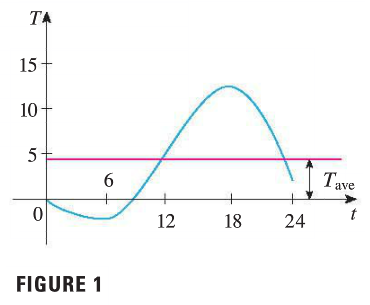
\includegraphics[scale=0.37]{6-5figure1.png}\]
  In general, is there a number $c$ at which the value of a function $f$ is exactly equal to the average value of the function, i.e., $f(c) = f_{\text{ave}}$? The following theorem says, YES, for continuous functions.\\
  \indent
  
  
\fbox{
  \parbox{\textwidth}{
  \vspace{5pt} \textbf{The Mean Value Theorem for Integrals:} If $f$ is continuous on $[a,b]$, then there exists a number $c$ in $[a,b]$ such that\\
  \indent
  
  \[\text{ }\]
  
  \indent
  
  \[\text{ }\]
  
  
  }}
  \indent\\
  
  \newpage
  The geometric interpretation of the Mean Value Theorem for Integrals is that, for \textit{positive} functions $f$, there is a number $c$ such that the rectangle with base $[a,b]$ and height $f(c)$ has the same area as the region under the graph of $f$ from $a$ to $b$. (See Figure 2)
  
  \[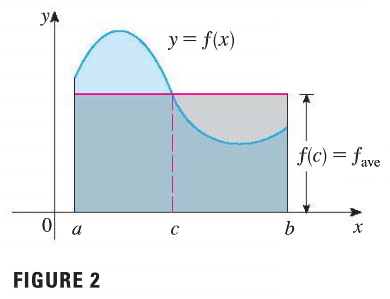
\includegraphics[scale=.37]{6-5figure2a.png} \quad \quad 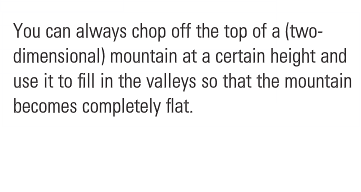
\includegraphics[scale=0.5]{6-5figure2b.png}\]


\indent

\underline{Example 2}: Since $f(x) = 1+x^2$ is continuous on the interval $[-1,2]$, the Mean Value Theorem for Integrals says there is a number $c$ in $[-1,2]$ such that:\\
\indent

\[\text{ }\]

\[\text{ }\]

In this particular case we can find $c$ explicitly. From Example 1, we know that $f_{\text{ave}}= \underline{\hspace{0.3in}}$, so we have:\\
\indent

\vspace{0.6in}

So in this case there happen to be two numbers $c=\underline{\hspace{0.4in}}$ in the interval $[-1,2]$ that work in the Mean Value Theorem for Integrals.\\
\indent\\
\indent\\
\indent

\underline{Example 3}: Show that the average velocity of a car over a time interval $[t_1,t_2]$ is the same as the average of its velocities during the trip.\\
\indent

SOLUTION: If $s(t)$ is the displacement of the car at time $t$, then, by definition, the average velocity of the car over the interval is:\\
\indent

\[\text{ }\]
\indent\\
\indent

On the other hand, the average value of the velocity function on the interval is:

\vspace{1.5in}



%----------------------------------------------------------------------------------------

\end{document}